\chapter{Uroczyste Requiem}

\section{Przygotowanie}%

\begin{itemize}
	\item Ołtarz główny:
		\begin{itemize}
			\item bez kwiatów
			\item mszał otwarty
			\item katafalk
			\item 4 świeczniki z \textcolor{orange}{żółtymi} świecami
			\item przy sedilli dodatkowe dwa miejsca dla akolitów
			\item \textcolor{violet}{fioletowe} antepedium (?)
		\end{itemize}
	\item Kredencja:
		\begin{itemize}
			\item kielich nakryty \textbf{czarnym} welonem
			\item brak welonu naramiennego dla \ss
			\item ampułki
			\item lawaterz, ręczniczek
			\item dzwonki
			\item lekcjonarz/ewangeliarz
			\item dwie pateny komunijne (?)
			\item dwie świece sanctusowe (?)
			\item kociołek, aspergil
			\item rytuał
		\end{itemize}
	\item Zakrystia/kaplica:
		\begin{itemize}
			\item dla \ii: humerał, alba simplex, \textbf{czarne
				cingulum, czarny ornat, stuła, manipularz},
				biret
			\item dla \dd: humerał, alba simplex, \textbf{czarne cingulum,
				czarna dalmatyka, stuła, manipularz}, biret
			\item dla \ss: humerał, alba simplex, \textbf{czarne cingulum,
				czarna tunicella, (manipularz)}, biret
			\item \textbf{czarna kapa}
			\item krzyż procesyjny
			\item trybularz, łódka
			\item akolitki (z \textcolor{orange}{żółtymi} świecami)
		\end{itemize}
\end{itemize}

\section{Pochód do ołtarza}

\begin{itemize}
	\item procesja wejścia przebiega w następującym porządku:
		\begin{center}
			\tt~~~\cc2 \\
			\aa2 ~~ \ding{63} ~~ \aa1\\
			ministranci\\
			\cc1 \\
			\ss \\
			\dd \\
			\ii 
		\end{center}
    \item \aa\aa~ wnoszą zapalone akolitki w procesji wejścia oraz wynoszą po
	    zakończeniu mszy; w czasie mszy akolitki stoją zapalone na
	    kredencji i nie są używane na Ewangelię
    \item \tt~ nie wnosi kadzielnicy w procesji wejścia
    \item \ii, \dd~ i \ss~ oddają birety \cc1, a następnie przyklękają na jego znak
    \item podczas mszy opuszcza się wszystkie pocałunki
\end{itemize}

\section{Od modlitwy u stopni do sekwencji}

\begin{itemize}
	\item  \cc1 daje znak dla asysty do klęknięcia
	\item następują modlitwy u stopni z pominięciem psalmu 42 \textit{Iudica me}
	\item \ii~wstępuje po stopniach ołtarza i go całuje
	\item pomija się okadzenie, przejście od razu na Introit
	\item \ii~kładzie lewą rękę na ołtarzu, a prawą czyni znak krzyża nad
		otwartym mszałem; czyta \textit{Introit}
	\item cała asysta opuszcza znak krzyża
	\item \ii, \dd, \ss~i \cc1 recytują \textit{Kyrie}	
	\item po zakończeniu recytacji \dd~i \ss~stają za \ii, a jeśli śpiew się
		przedłuża schodzą krótką drogą do sedilli
	\item pod koniec Kyrie \ii, \dd~i \ss~przechodzą na środek
	\item \ii~całuje ołtarz, śpiewa pozdrowienie i razem z \dd~i \ss~przechodzą
		na stronę lekcji
	\item podczas kolekty, od \textit{Dominus Vobiscum} aż do
		\textit{Amen}, cała asysta niższa klęczy
	\item pod koniec oracji \cc1 zabiera z kredencji lekcjonarz i przekazuje
		go \ss
	\item \cc1 i \ss~przyklękają na osi ołtarza i odchodzą na miejsce śpiewania
		lekcji, gdzie \cc1 staje po lewej stronie \ss~(bliżej osi ołtarza)
	\item \dd~zajmuje miejsce przy mszale
	\item \ss~śpiewa lekcję, którą \ii~czyta cicho w mszale
	\item \ss~wraca z \cc1, przyklękają na osi ołtarza
	\item \cc1 odbiera lekcjonarz, \ss~nie podchodzi po błogosławieństwo, tylko
		razem z \dd~stają jak na \textit{Introit}
	\item \ii~recytuje sekwencję, \cc1 asystuje przy mszale
	\item po zakończeniu recytacji asysta wyższa schodzi krótką drogą do
		sedilli
	\item około słów \textit{Qui Mariam absolvisti}, na znak \cc1 wracają do ołtarza
		przyklękając na środkui
	\item \ii~wchodzi po stopniach i staje pośrodku ołtarza
\end{itemize}

\section{Ewangelia}

\begin{itemize}
	\item \cc1 podaje \dd~ewangeliarz
	\item w tym czasie \ss~wchodzi na suppedaneum po stronie lekcji, skąd
		zabiera mszał i wraca z nim przed stopnie, po lewej stronie \dd
	\item \dd~i \ss~przyklękają i wchodzą po stopniach, każdy na swoją stronę
	\item \ss~stawia mszał po stronie ewangelii, a \dd~kładzie ewangeliarz na
		środku ołtarza
	\item w tym czasie przed ołtarzem ustawiają się \aa1, \aa2 (bez akolitek),
		\tt~(bez kadzielnicy) oraz \cc1
	\item \ss~schodzi przed stopnie i zajmuje miejsce w pierwszym rzędzie po
		stronie ewangelii
	\item \dd~klęka na skraju suppedaneum, na prawo od \ii~i odmawia
		\textit{Munda cor meum}, następnie wstaje, zabiera ewangeliarz,
		skłania się i nie prosząc o błogosławieństwo schodzi przed
		stopnie po stronie lekcji; porządek wygląda następująco:
		\begin{center}
			|\_\_\_\_\_\_\_\_\_\_\_\_\_\_\_\_\_\_\_\_\_\_\_\_\_\_|\\
			\ss~~~~\dd\\
			\cc1~~~~\tt\\
			\aa2~~~~\aa1
		\end{center}
	\item wszyscy przed stopniami przyklękają i odchodzą na miejsce proklamacji
		ewangelii, gdzie ustawiają się jak zwykle
	\item pomija się okadzenie, \dd~rozpoczyna śpiew Ewangelii
	\item po zakończeniu proklamacji nie okadza się celebransa
	\item \ss~oddaje ewangeliarz \cc1
	\item wszyscy wracają przed ołtarz w tym samym porządku
	\item na znak \cc1 przyklękają i wracają na swoje miejsca: \dd~i \ss~na stopniach
		za \ii, \aa\aa~ do kredencji, \tt~idzie przygotować kadzielnicę (która
		powinna być rozpalona już wcześniej), a \cc1 odnosi ewangeliarz na
		kredencję i staje na swoim miejscu
	\item w tym miejscu liturgii nie przewiduje się kazania
\end{itemize}

\section{Ofiarowanie}

\begin{itemize}
	\item \ii~całuje ołtarz i śpiewa \textit{Dominus vobiscum} oraz
		\textit{Oremus}
	\item \dd~wchodzi na suppedaneum i staje po prawej stronie \ii~(bez
		przyklęknięcia)
	\item \ss~i \cc1 przyklękają na środku i odchodzą do kredencji
	\item \ss~bierze kielich przykryty welonem i bursą, i zanosi go na
		ołtarz, sam jednak nie zakłada welonu naramiennego, gdyż nie
		trzyma pateny
	\item \dd~rozkłada korporał na ołtarzu, \ss~rozbiera kielich
	\item \aa1 przynosi na ołtarz ampułki, odbiera od \ss~welon kielichowy i
		odnosi go na kredencję
	\item jeśli może, \ss~nalewa wody do kielicha, jeśli nie, robi to \dd, w
		obu przypadkach jednak nie prosząc \ii~o błogosławieństwo
	\item \aa1 zabiera ampułki z ołtarza na kredencję
	\item \tt~przychodzi z rozpaloną kadzielnicą i łódką
	\item \ss~nie trzyma pateny, więc przechodzi na lewą stronę \ii,
		przyklękając na środku na najniższym stopniu
	\item \dd~chowa patenę pod korporałem, jak na mszy śpiewanej
	\item następuje okadzenie; \cc1 odbiera łódkę od \tt~i razem wchodzą po
		stopniach
	\item \cc1 podaje łódkę \dd, następuje zasypanie
	\item \dd~oddaje łódkę \cc1, a odbiera kadzielnicę od \tt
	\item \cc1 i \tt~schodzą ze stopni
	\item okadzenie ołtarza przebiega jak zwykle
	\item \cc1 przechodzi na stronę ewangelii i w odpowiedniej chwili ściąga
		z ołtarza mszał, po okadzeniu odnosi go i zostaje przy mszale
	\item po okadzeniu ołtarza okadzony zostaje jedynie \ii~(przez \dd~i \ss)
	\item \tt~wynosi kadzielnicę bez dalszych okadzeń, idzie na środek
		i czeka aż dołączą do niego ceroferariusze wraz z \cc2
	\item \cc2 wyprowadza ceroferariuszy (dwóch lub czterech), którzy idą
		przygotować pochodnie – przyklękają parami na środku i odchodzą
	\item \dd~i \ss~stają w linii za \ii~(jak na oracje)
	\item \aa\aa~ dokonują obmycia rąk \ii~(lavabo)
	\item \ii, \dd~i \ss~przechodzą na środek, wciąż stojąc w linii
	\item \dd~odpowiada na \textit{Orate, fratres}
\end{itemize}

\section{Prefacja i Kanon Rzymski}

\begin{itemize}
	\item następuje prefacja
	\item pod koniec prefacji \cc1 skłania się do \dd~i \ss, po czym odchodzi od
		mszału i idzie na swoje miejsce
	\item \dd~i \ss~wchodzą na suppedaneum i pochyleni recytują \textit{Sanctus}
		razem z \ii~(\dd~po prawej, \ss~po lewej przy mszale)
	\item po zakończeniu recytacji \dd~i \ss~stają na stopniach za \ii~i
		przyklękają
	\item \dd~przechodzi na stronę ewangelii i asystuje przy mszale
	\item \ss~zostaje przed najniższym stopniem i stoi tam ze złożonymi rękami
	\item do ołtarza przychodzą \cc2, \tt~oraz ceroferariusze
	\item przyklękają na środku, \tt~odchodzi do kredencji, a \cc2 na swoje
		miejsce
	\item w czasie Kanonu Rzymskiego cała asysta niższa klęczy – od
		zakończenia recytacji \textit{Sanctus} aż do końcowego
		\textit{Amen}, dlatego na znak \cc2 wszyscy klękają na oba
		kolana, w tym ceroferariusze na środku \item na słowa \textit{Quam
		oblationem} \dd~schodzi na środek, przyklęka i przechodzi na
		prawą stronę \ii
	\item w tym czasie \ss, nie przyklękając, przechodzi wzdłuż stopni na
		stronę lekcji, gdzie odbiera przy kredencji zasypaną
		kadzielnicę od \tt, a następnie klęka na najniższym stopniu; \cc1
		klęka w tym samym momencie
	\item podczas podniesienia \ss~okadza Najświętszy Sakrament
	\item po konsekracji \dd~wraca do mszału na lewą stronę \ii, z
		przyklęknięciami po obu stronach, natomiast \ss~oddaje
		kadzielnicę \tt~i wraca na środek, gdzie przyklęka i stoi aż do
		\textit{Pax Domini sit semper vobiscum}
	\item jak zwykle po słowach \textit{Nobis quoque peccatoribus} \dd~przyklęka przy
		mszale, przechodzi na prawą stronę \ii~i znów przyklęka
	\item \cc1 przechodzi na środek, przyklęka (za plecami \ss) i zajmuje
		miejsce przy mszale, gdzie znów przyklęka (równocześnie z \dd)
	\item po zakończeniu Kanonu wszyscy wstają na znak \cc2
	\item ceroferariusze przyklękają na środku razem z \cc2 i \tt, a następnie
		razem z nimi wychodzą
\end{itemize}

\section{Od \textit{Pater Noster} do końca Mszy}

\begin{itemize}
	\item \ii~rozpoczyna śpiew \textit{Pater noster}, \dd~przyklęka,
		schodzi na stopień za \ii~i tam znów przyklęka
	\item na słowa \textit{Et dimitte nobis} \dd~przyklęka, wraca na prawą
		stronę \ii~i bez pocałunku podaje mu patenę; w tym czasie
		\ss~pozostaje na swoim miejscu
	\item na słowa \textit{Pax Domini sit semper vobiscum} \ss~i \cc1 przyklękają, a
		następnie \ss~zajmuje miejsce przy mszale, \cc1 zaś odchodzi na
		swoje miejsce
	\item \ii, \dd~i \ss~recytują \textit{Agnus Dei} w zmienionej formie,
		stąd nie biją się w pierś
	\item opuszcza się przekazanie pocałunku pokoju, więc po zakończeniu
		recytacji \dd~i \ss~zamieniają się miejscami przyklękając przed i
		po
	\item \cc2, \tt~i ceroferariusze wracają do ołtarza i razem z pozostałymi
		ministrantami formują procesję komunijną
	\item \cc1 daje znak do przyklęknięcia, a następnie do klęknięcia
	\item następuje komunia wiernych
	\item po komunii \aa1 zanosi na ołtarz ampułki, a po ablucjach je zabiera
	\item \dd~bierze mszał, który przenosi na stronę lekcji, \ss~bierze palkę,
		którą przenosi na stronę ewangelii, przyklękają na środku na
		swoich stopniach
	\item \aa2 zanosi welon kielichowy na stronę ewangelii i podaje go \ss
	\item \cc1 przechodzi do mszału
	\item \ss~odnosi kielich na kredencję
	\item \ii, \dd~i \ss~stają w jednej linii, następuje \textit{Communio},
		wezwanie (na środku) i pokomunia (znów po stronie lekcji)
	\item \cc1 zamyka mszał
	\item \ii, \dd~i \ss~wracają na środek, \ii~całuje ołtarz i śpiewa
		\textit{Dominus vobiscum}
	\item \dd~wciąż zwrócony w stronę ołtarza śpiewa \textit{Requiescant in
		pace}, na co odpowiada się \textit{Amen}
	\item \ii~odmawia \textit{Placeat}, pomija się błogosławieństwo i Ostatnią
		Ewangelię, ponieważ następują absolucje
\end{itemize}

\section{Absolucje}

\begin{itemize}
	\item \ii, \dd~i \ss~odchodzą do sedilli
	\item Z przynosi z zakrystii czarną kapę
	\item \dd~i \ss~z pomocą Z asystują \ii~przy zdejmowaniu ornatu i manipularza
		oraz zakładaniu kapy
	\item \dd~i \ss~zdejmują manipularze z pomocą \aa\aa~
	\item \aa\aa~ biorą akolitki, krucyferariusz podaje krzyż procesyjny \ss
	\item M1 bierze rytuał, M2 bierze kropidło
	\item \tt~przychodzi z kadzielnicą
	\item \ss~trzymając krzyż staje z \aa\aa~ u wezgłowia katafalku, pozostawiając
		odstęp
	\item M1, M2 oraz \tt~stają przy stopniach ołtarzowych po stronie lekcji,
		zwróceni w stronę nawy
	\item \ii~staje w nogach katafalku, mając \dd~po swojej prawej, a \cc1 po
		lewej stronie, zwróceni w stronę nawy (patrz Rys.
		\ref{fig:requiem})
		\begin{figure}[h]
			\centering
			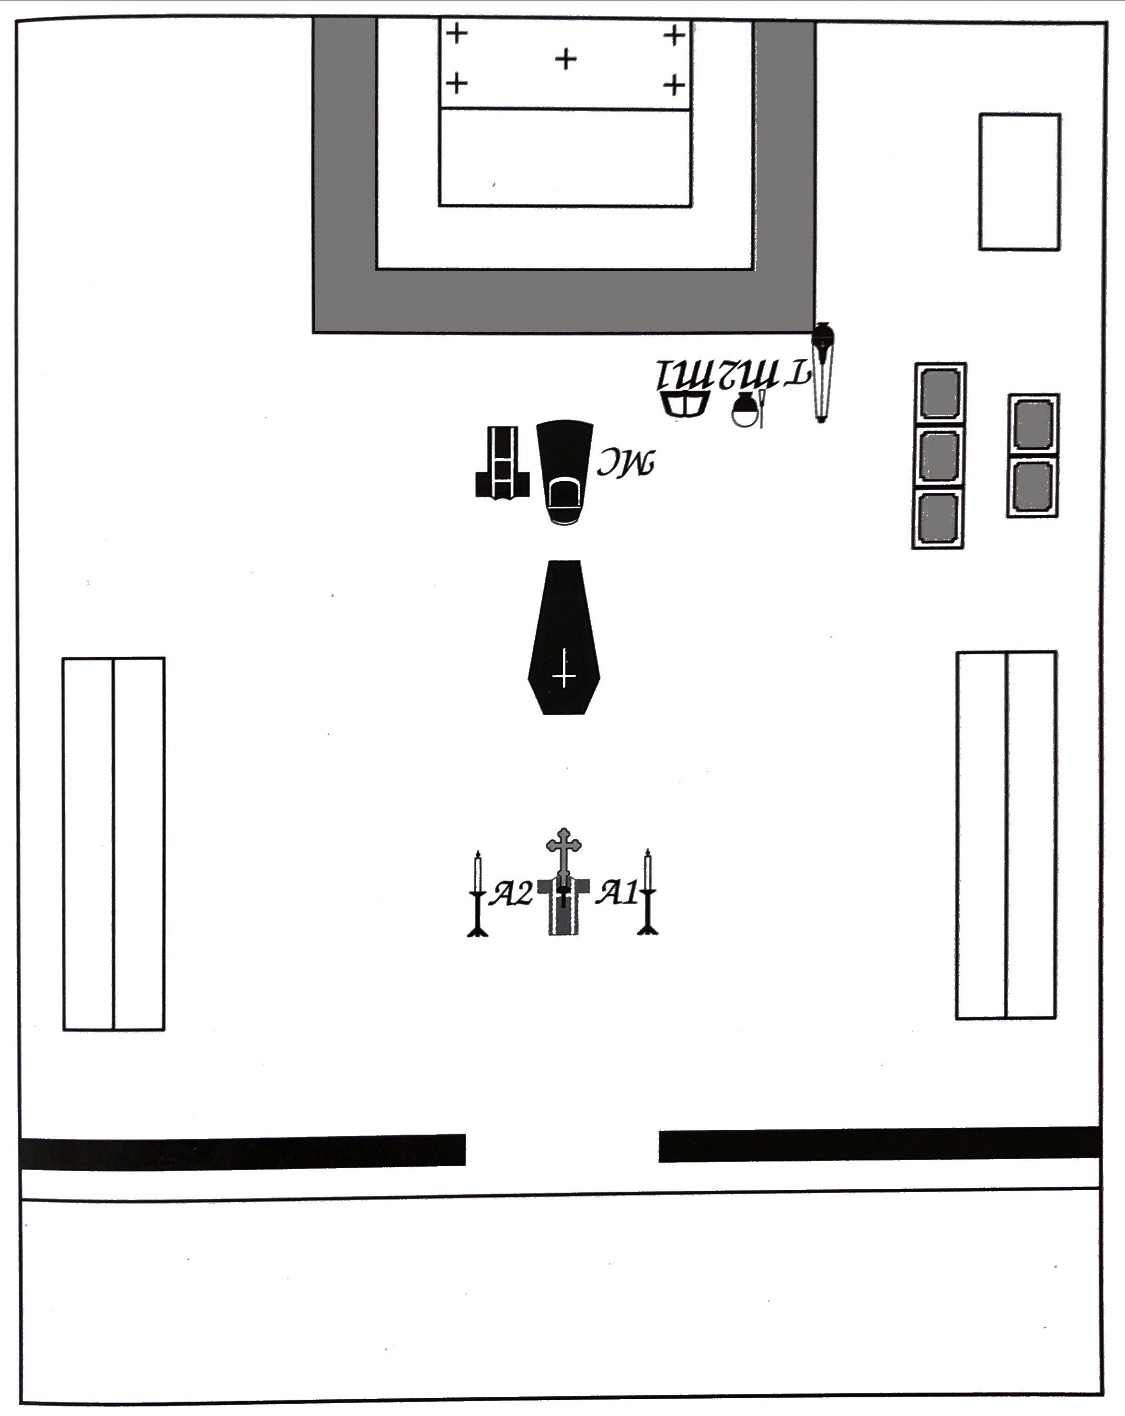
\includegraphics[width=0.8\textwidth]{Figures/requiem.jpg}
			\caption{Ustawienie przy katafalku}
			\label{fig:requiem}
		\end{figure}
	\item ponieważ nie ma ciała, opuszcza się modlitwę \textit{Non intres}
	\item schola rozpoczyna śpiew responsorium \textit{Libera me}
	\item podczas powtórzenia pierwszego wersetu następuje zasypanie
		kadzidła
	\item \tt~oraz \cc1 przechodzą razem na stronę ewangelii
	\item \tt~podaje łódkę \dd~i podnosi kadzielnicę do zasypania
	\item \dd~prosi \textit{Benedicite, Pater reverende}
	\item \ii~zasypuje 3 razy, błogosławiąc w zwykły sposób (bez pocałunków)
	\item \tt~odbiera łódkę i wraca z kadzielnicą na swoje miejsce
	\item \cc1 wraca na lewą stronę \ii
	\item po responsorium śpiewa się dialog \textit{Kyrie, eleison}
	\item M1 podchodzi z rytuałem, staje na prawo od \ii, przed \dd
	\item \ii~zwraca się do zgromadzonych i wspólnie recytują \textit{Ojcze
		nasz}
	\item M1 odchodzi, podchodzi M2 z kropidłem, które podaje \dd
	\item \dd~bez pocałunków podaje kropidło \ii
	\item \dd~trzyma prawą połę kapy, \ii~zaś kropi katafalk najpierw
		trzykrotnie z prawej strony (od strony ewangelii), nie
		zatrzymując się
	\item przechodząc przed krzyżem \ii~lekko się skłania, a \dd~przyklęka
	\item \ii~kropi katafalk trzykrotnie z lewej strony, również się nie
		zatrzymując
	\item po powrocie przed ołtarz obaj przyklękają przed Najświętszym
		Sakramentem
	\item ustawiają się na powrót przed katafalkiem, \ii~oddaje kropidło \dd, a
		ten M1
	\item M1 odchodzi z kropidłem, podchodzi \tt~z kadzielnicą
	\item \tt~podaje kadzielnicę \dd, a ten \ii
	\item okadzenie następuje analogicznie do pokropienia
	\item podchodzi M1 z rytuałem, \ii~śpiewa wezwania oraz modlitwę
		\textit{Absolve}
	\item \ii~prawą ręką czyni znak krzyża nad katafalkiem i śpiewa wezwania
	\item na zakończenie śpiewa się antyfonę \textit{Salve, Regina}
	\item \ss~oddaje krzyż krucyferariuszowi
	\item ustawia się procesja do wyjścia, w porządku analogicznym jak na
		wejście
\end{itemize}
